\section{Experimental results}
\label{sec:ch5sec5}

\subsection{Used datasets}

The segmentation was performed on a homemade manually labeled dataset which includes a subset of IAM and RIMES images and school notebooks scans (some of them shown in Figure \ref{FigCustomDS}). It was considered crucial to train the model on as many real world samples as possible, because the quality of the final predicted text is tightly linked to the state of the segmentation. 

\begin{figure}[htbp]
    \centering
        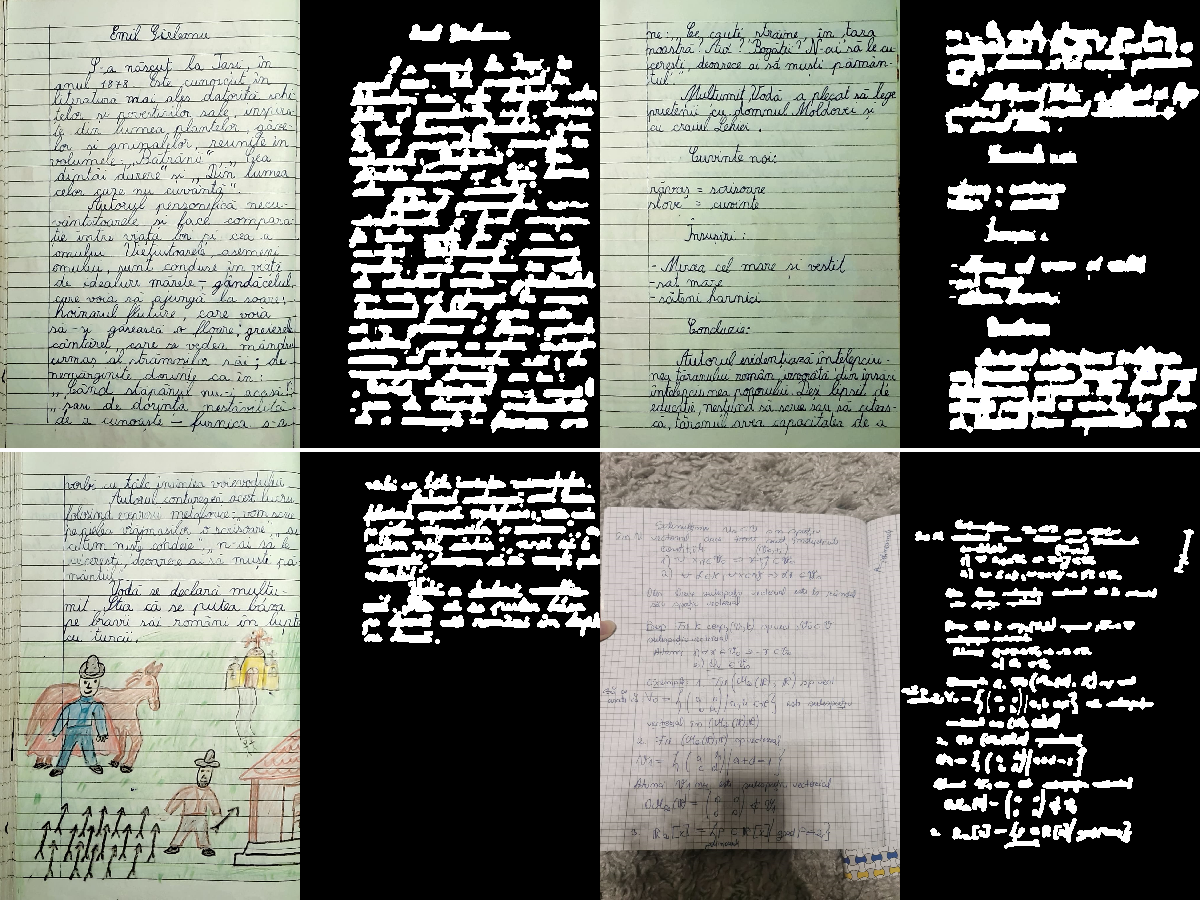
\includegraphics[scale=0.6]{figures/custom_db.png}
    \caption{Samples from own segmentation dataset}    
    \label{FigCustomDS}
\end{figure}

For the recognition part, IAM lines dataset constitutes the main source of training data, with a minor contribution consisting of own crafted samples.



\subsection{Evaluation metrics}

The quality of the model mask output is measured by the IoU \cite{iou} and Dice \cite{dice} metrics:
$$ IoU(R,P) = \frac{|R \cap P|}{|R \cup P|} = \frac{TP}{TP+FP+FN} $$
$$ Dice(R,P) = \frac{2|R \cap P|}{|R| + |P|} = \frac{2 TP}{2TP+FP+FN},  $$
where $R$ and $P$ are the real and the predicted masks.

For the line segmentation task, the precision and recall variants introduced in the work of Berat et al. were used for evaluation \cite{segmChallenging}, where the smallest measure unit was chosen to be pixel instead of the connected component:

$$Recall(l_i) = \sum_{p \in P, p\cap l_i \neq \emptyset} \frac{|p \cap l_i|-1}{|l_i|-1}$$
$$Precision(l_i) = \frac{ (\sum_{p\in P, \space p\cap l_i \neq \emptyset} |p\cap l_i|)-1}{
(\sum_{p\in P, \space p\cap l_i \neq \emptyset} |p|)-1},$$
where $l_i \in R$ are the ground truth lines and $p\in P$ are the labeled lines on the predicted mask.
By comparing these formulas with their counterparts from section \ref{subsubsec:ch3sec2subsec4subsubsec3}, one can infer a similar method to compute the per-line segmentation accuracy:

$$Accuracy(l_i) = \frac{\sum_{p \in P, p\cap l_i \neq \emptyset}(|p \cap l_i| + |\overline{p\cup l_i}|)-1}{\sum_{p \in P, p\cap l_i \neq \emptyset} |\Omega|-1},$$
where $|\Omega|$ was chosen to be the minimum area rectangle that includes $R$ and $P$, and $\overline{p\cup l_i}=\Omega \setminus (p \cup l_i)$.

On the recognition part, the Character Error Rate (CER) metric was used to va\-lidate the performance of the model. It computes the edit distance between the ground truth and the prediction by counting the 
minimum number of insertions ($\#I$), deletions ($\#D$) and substritutions ($\#S$) required to transform a sequence into another \cite{cer}:
$$CER = \frac{\#I+\#D+\#S}{\#characters\_count}$$

\subsection{Training session}


The segmentation model's architecture is the U-Net with a LSTM layer in the middle which was visually depicted in Figure \ref{FigSegArch}. A more technical description is provided by Figure \ref{FigSegModelSumm}. It is useful to note that the repetitive structures of layers on both the encoder and decoder part have been combined into two subclassed layer blocks (visible in Figure \ref{FigEncDecBlock}) for an improved clarity and better comprehension. Thus, the U-net would look like a simplified stack of encoder blocks and decoder blocks.

This model was trained using the binary crossentropy loss and the Adam optimizer. The learning rate starts from $10^{-3}$ and decreases gradually by a factor of $0.8$ (but no lower than $10^{-6}$) when the model keeps making no progress. The dataset was augmented by performing random scaling, rotation and perspective transform to the images. It contains 138 samples which are majoritarly manually segmented IAM images, but also RIMES and custom images. The small size of the dataset is complemented by the fact that tiling would significantly increase volume of train data. What segmentation model actually sees for each sample image are the sixteen 64x64px images resulting from tiling (or $80\times80$px if the tiles padded), and additional randomly cropped tiles that do not align with the 4x4 grid. This is done in order to try make the model as position independent as possible. The training  reaches its limits after at most 140 short epochs with a simple setup of 400 steps per epoch and a batch size of 1. 

\begin{figure}[htbp]
\begin{lstlisting}[escapeinside={(*}{*)}, basicstyle=\tiny, xleftmargin=.15\textwidth, xrightmargin=.15\textwidth]
____________________________________________________________________________
 Layer (type)                    Output Shape          inputs        Param #
============================================================================
 x_input (Input)                 (None, 64, 64,  1)                     
 enc_block (EncBlock) (see Figure *\ref{FigEncDecBlock}*)        (None, 32, 32,  4)     x_input          188
 enc_block_1 (EncBlock)          (None, 16, 16,  8)     enc_block        880
 enc_block_2 (EncBlock)          (None,  8,  8, 16)     enc_block_1     3488
 enc_block_3 (EncBlock)          (None,  4,  4, 32)     enc_block_2    13888
 enc_block_4 (EncBlock)          (None,  2,  2, 64)     enc_block_3    55394
 reshape (Reshape)               (None,  64, 4)         enc_block_4        0
 bidirectional (Bidirectional)   (None,  64, 4)         reshape          112
 reshape_1 (Reshape              (None,  2,  2, 64)     bidirectional      0
 dec_block (DecBlock)            (None,  4,  4, 64)     reshape_1,    147644
                                                        enc_block_4
 dec_block_1 (DecBlock)          (None,  8,  8, 32)     dec_block,     46176
                                                        enc_block_3
 dec_block_2 (DecBlock)          (None, 16,  16, 16)    dec_block_1,    11568
                                                        enc_block_2
 dec_block_3 (DecBlock)          (None, 32,  32, 8)     dec_block_2,     2904
                                                        enc_block_1
 dec_block_4 (DecBlock)          (None, 64,  64, 4)     dec_block_3,      732
                                                        enc_block
 conv2d (Conv2D) 1x1             (None, 64,  64, 3)     dec_block_4,       37
=============================================================================
Total params: 8,471,762
Trainable params: 8,471,762
Non-trainable params: 0
_____________________________________________________________________________
\end{lstlisting}
\caption{Segmentation model}
\label{FigSegModelSumm}
\end{figure}

\begin{figure}[htbp]
    \centering
        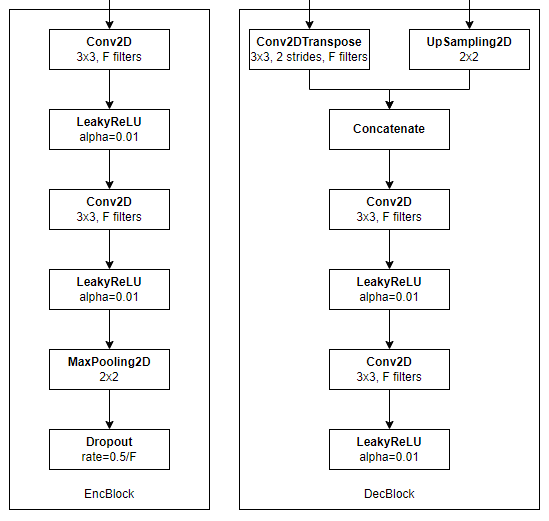
\includegraphics[scale=0.4]{figures/encdec_block.PNG}
    \caption{Encode and decode block}    
    \label{FigEncDecBlock}
\end{figure}


The recognition model (Figure \ref{FigRecModel}) features previously mentioned CNN-LSTM architecture. It was trained for $100$ epochs with a batch size of $5$, at a constant learning rate of $10^{-3}$. The training process takes a similar route to the one described in Hemanth et al.'s  paper \cite{cnnrnn}. The recognition model is encapsulated in a driver model used for training use only (Figure \ref{FigRecTrainModel}), which feeds the ground truth values needed for the CTC loss, like the padded output sequence, the original text length and   the number of character labels. It was trained on the 13353 presegmented images from the IAM lines dataset (train/validation split 90\%/10\%), rescaled to fit in a 1024x64px box, grouped in batches of 5. The model outputs 128 sequences of probabilities for 92 classes, each one corresponding to a text character. They are the usual 81 characters found in IAM dataset (plus the "\#" character to replace unrecognizable text/ "erased" by cutting it with a line) ordered by their ASCII code with 10 additional labels to account for Romanian diacritics (5 lowercase and 5 uppercase).

\begin{figure}[htbp]
\begin{lstlisting}[escapeinside={(*}{*)}, basicstyle=\tiny, xleftmargin=.1\textwidth, xrightmargin=.1\textwidth]
__________________________________________________________________________________
 Layer (type)                   Parameters        Output Shape             Param #
==================================================================================
 x_input (Input)                                   (None,  64, 1024,  64)        0
 conv2d (Conv2D)                 5x5, 64 filters   (None,  64, 1024,  64)     1664
 leaky_re_lu (LeakyReLU)         alpha=0.01        (None,  64, 1024,  64)        0
 max_pooling2d (MaxPooling2D)    2x2               (None,  32,  512,  64)        0
 conv2d_1 (Conv2D)               5x5, 128 filters  (None,  32,  512, 128)   204928
 leaky_re_lu_1 (LeakyReLU)       alpha=0.01        (None,  32,  512, 128)        0
 max_pooling2d_1 (MaxPooling2D)  2x1               (None,  16,  512, 128)        0
 conv2d_2 (Conv2D)               3x3, 128 filters  (None,  16,  512, 128)   147584
 leaky_re_lu_2 (LeakyReLU)       alpha=0.01        (None,  16,  512, 128)        0
 max_pooling2d_2 (MaxPooling2D)  2x2               (None,   8, 256, 128)         0
 conv2d_3 (Conv2D)               3x3, 256 filters  (None,   8, 256, 256)    295168
 leaky_re_lu_3 (LeakyReLU)       alpha=0.01        (None,   8, 256, 256)         0
 max_pooling2d_3 (MaxPooling2D)  2x2               (None,   4, 128, 256)         0
 conv2d_4 (Conv2D)               3x3, 512 filters  (None,   4, 128, 512)   1180160
 batch_normalization (Batch...)  mom=0.99,eps=1e-3 (None,   2, 128, 512)      2048
 leaky_re_lu_4 (LeakyReLU)       alpha=0.01        (None,   4, 128, 512)         0
 max_pooling2d_4 (MaxPooling2D)  2x2               (None,   2, 128, 512)         0 
 conv2d_5 (Conv2D)               3x3, 512 filters  (None,   2, 128, 512)   2359808
 leaky_re_lu_5 (LeakyReLU)       alpha=0.01        (None,   2, 128, 512)         0
 max_pooling2d_5 (MaxPooling2D)  2x1               (None,   1, 128, 512)         0
 reshape (Reshape)                                 (None, 128, 512)              0
 bidirectional (Bidirectional)                     (None, 128, 1024)       4198400
 reshape_1 (Reshape)                               (None, 128, 1, 1024)          0
 conv2d_6 (Conv2D)               1x1, 92 filters   (None, 128, 1, 92)        94300
 reshape_2 (Reshape)                               (None, 128, 92)               0
 softmax (Softmax)                                 (None, 128, 92)               0
==================================================================================
Total params: 8,484,060 (32.36 MB)
Trainable params: 8,483,036 (32.36 MB)
Non-trainable params: 1024 (4.00KB)
__________________________________________________________________________________
\end{lstlisting}
\caption{Recognition model}
\label{FigRecModel}
\end{figure}

\begin{figure}[htbp]
    \centering
        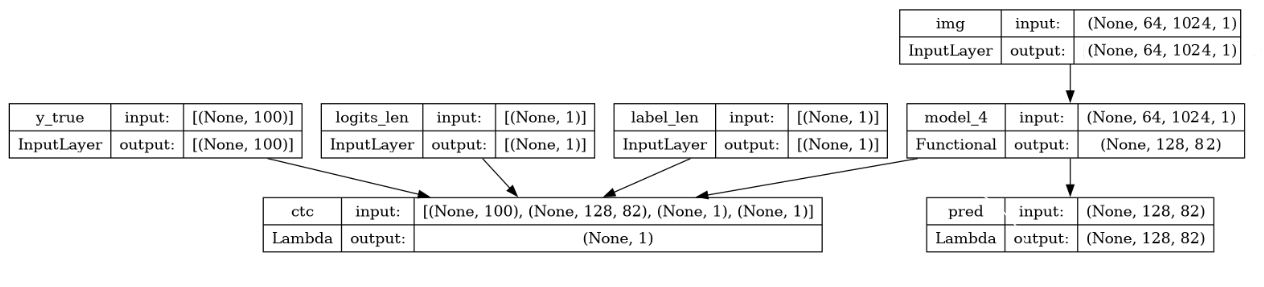
\includegraphics[scale=0.4]{figures/rec_train_model.png}
    \caption{Recognition training driver model}    
    \label{FigRecTrainModel}
\end{figure}

\subsection{Obtained performance}

The training process is summarized in Figure \ref{FigSegMetrics}. Table \ref{TableSegmentationMetrics} presents the performance of the segmentation model. The full mask metrics are computed on the model output after applying a threshold of $0.5$ to binarize the masks
and reflects how well the model fits on the used dataset. The previously mentioned line mask metrics describe the quality of the line segmentation algorithm. These metrics are computed once for each line by taking into account only those regions of the segmented mask that influence the detection of the given line. There results are eventually averaged, therefore the metrics such obtained should provide a more insightful measure of line segmentatin quality than the global metrics computed on the entire segmented mask. For a complete picture, table \ref{TableBeratSegResults} mentions the metrics obtained by the related Berat et al.'s segmentation method on "challenging historic images" of old handwritten texts \cite{segmChallenging}.

\begin{table}[htbp]
\begin{center}
\begin{tabular}
{|p{100pt}|p{50pt}|p{50pt}|}
\hline
 Metric  &  Train value & Validation value\\
\hline 
Accuracy & 0.9390 & 0.9664\\ \hline
Precision & 0.9254 & 0.9520 \\ \hline
Recall & 0.8379 & 0.8999 \\ \hline
F-Measure & 0.8794 & 0.9252 \\ \hline
IoU & 0.8626 & 0.9141 \\ \hline
Dice & 0.8768 & 0.9282 \\ \hline

\end{tabular}
\end{center}
\captionsetup{justification=centering,margin=1cm}
\caption{Segmentation model metrics on custom dataset \\ \small{(118 IAM pictures, 1 RIMES, 19 own images, 90\%/10\% train/test ratio)}}
\label{TableSegmentationMetrics}
\end{table}

\begin{table}[htbp]
\begin{center}
\begin{tabular}
{|p{100pt}|p{50pt}|p{50pt}|}
\hline
 Metric   & Value\\
\hline 
Precision & 0.78 \\ \hline
Recall & 0.82  \\ \hline
F-Measure & 0.80 \\ \hline

\end{tabular}
\end{center}
\captionsetup{justification=centering,margin=1cm}
\caption{Berat et al.'s segmentation results on historic Arabic manuscripts \cite{segmChallenging}}
\label{TableBeratSegResults}
\end{table}


\begin{table}[htbp]
\begin{center}
\begin{tabular}
{|p{100pt}|p{50pt}|p{50pt}|}
\hline
 Metric  &  Value \\
\hline 
Accuracy & 0.8377 \\ \hline
Precision & 0.4575 \\ \hline
Recall & 0.8560 \\ \hline
F-Measure & 0.5963 \\ \hline
IoU & 0.4031 \\ \hline
Dice & 0.5126 \\ \hline
\end{tabular}
\end{center}

\captionsetup{justification=centering,margin=1cm}
\caption{Lines segmentation metrics (validated on the entire IAM dataset)}
\label{TableSegmentationMetrics}
\end{table}

\begin{figure}[htbp]
    \centering
        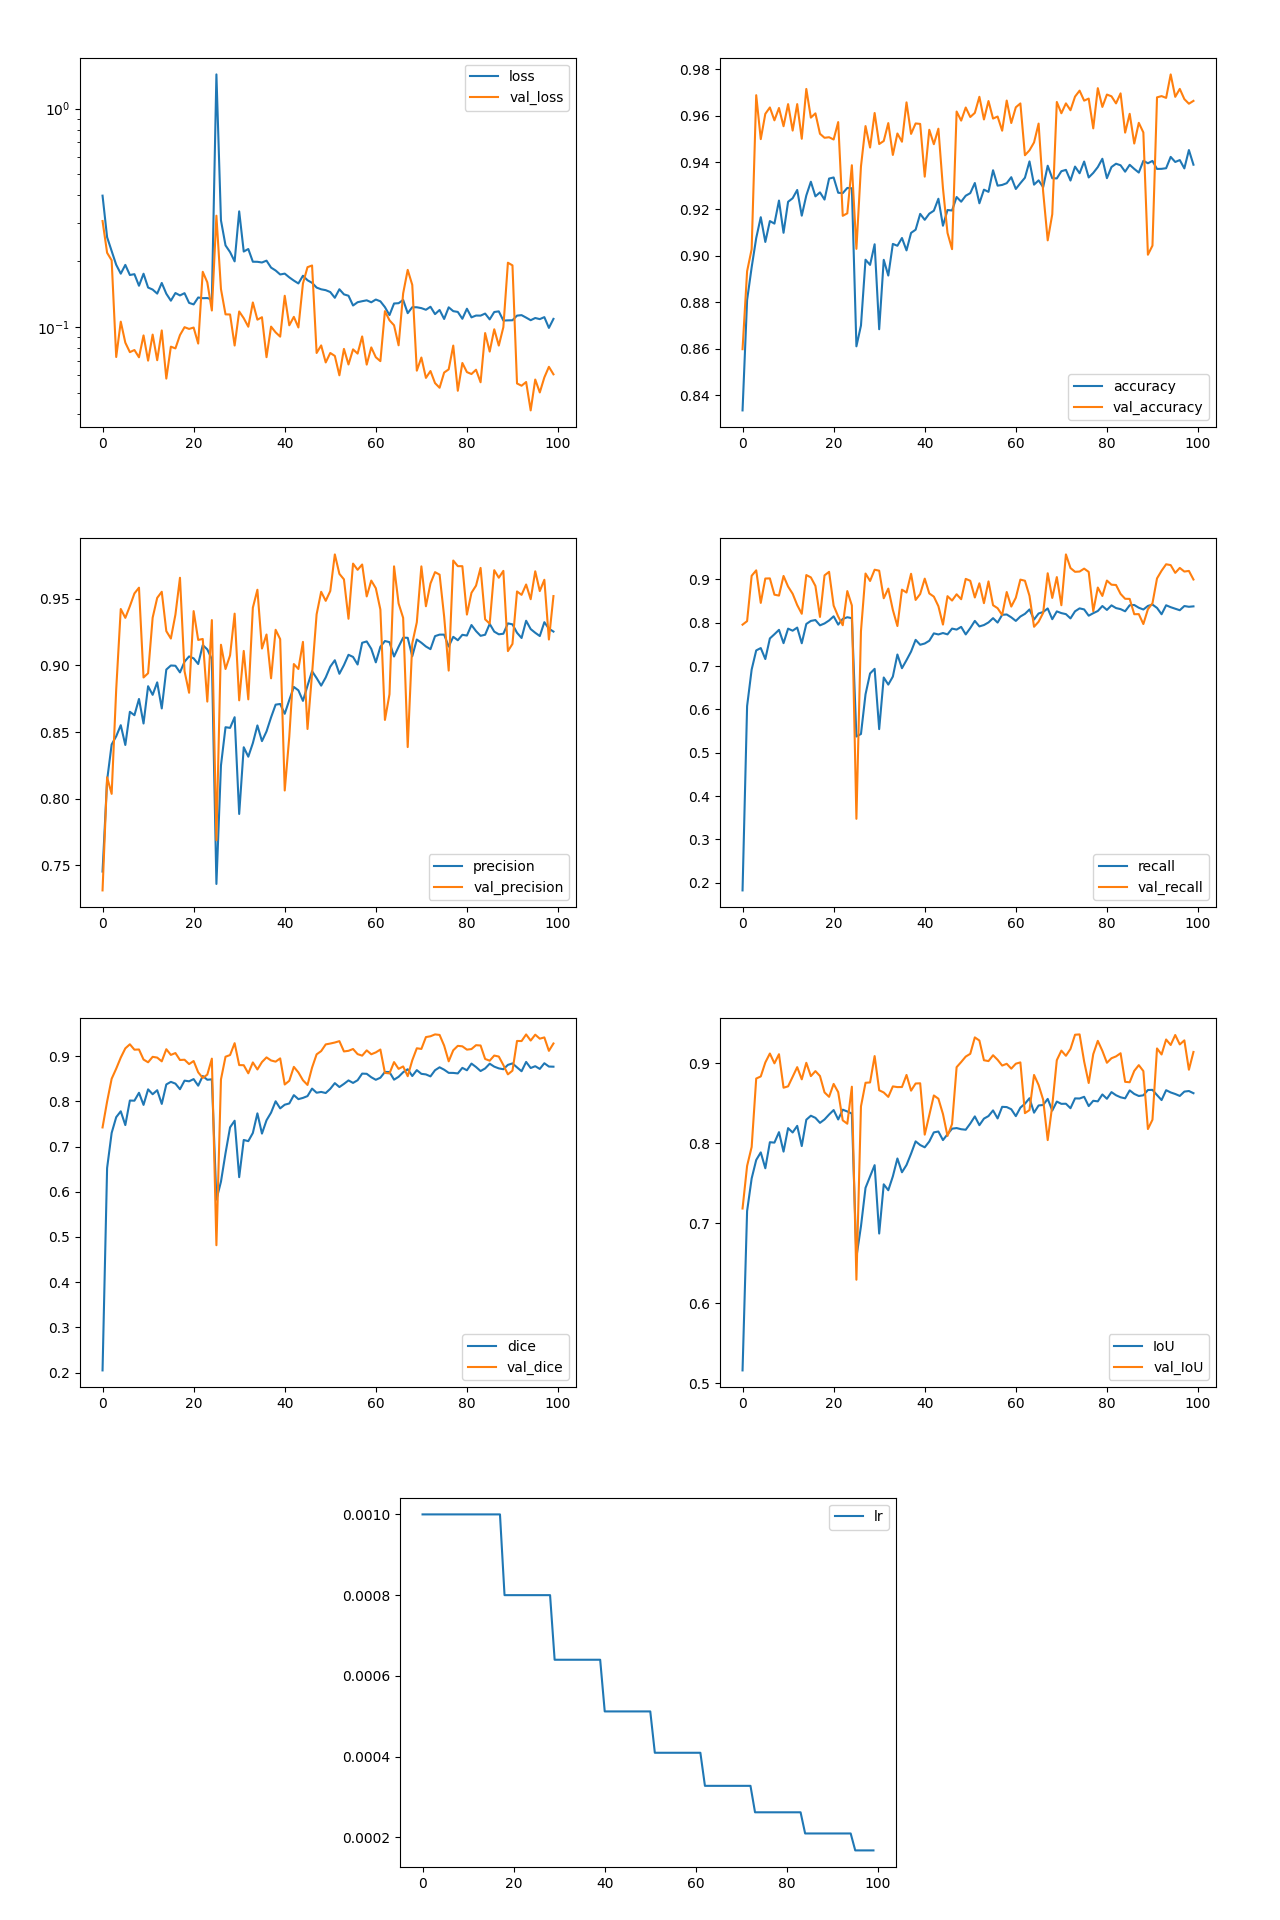
\includegraphics[scale=0.45]{figures/segtrain_results.png}
    \caption{Segmentation model metrics plot by epoch}    
    \label{FigSegMetrics}
\end{figure}


\begin{figure}[htbp]
    \centering
        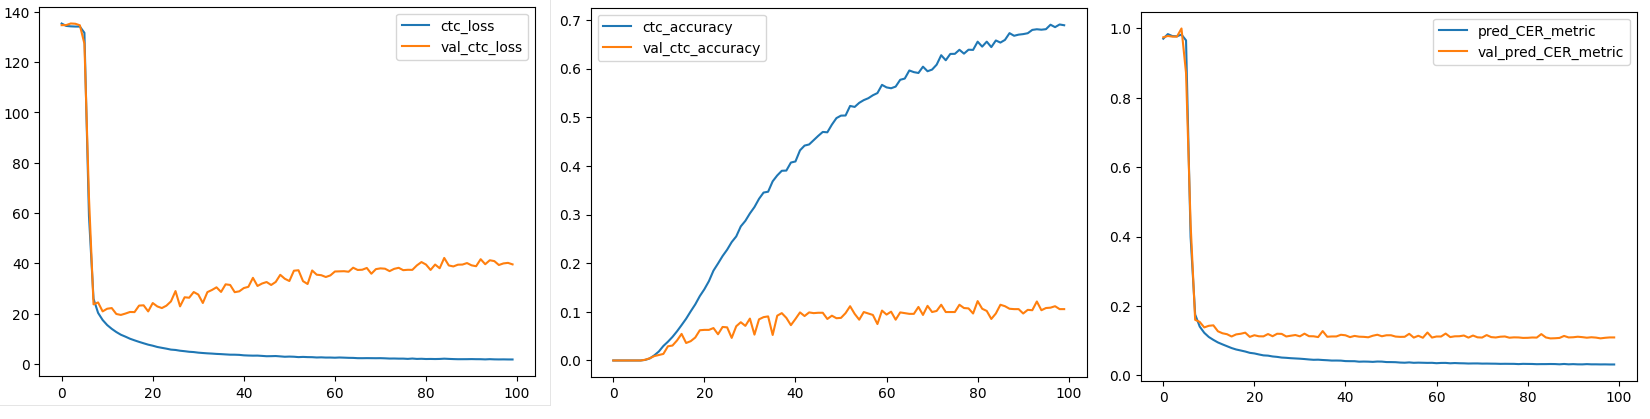
\includegraphics[scale=0.35]{figures/metrics_recog.png}
    \caption{Recognition model metrics per epoch (pure IAM lines dataset)}    
    \label{FigRecMetrics}
\end{figure}

\begin{figure}[htbp]
    \centering
        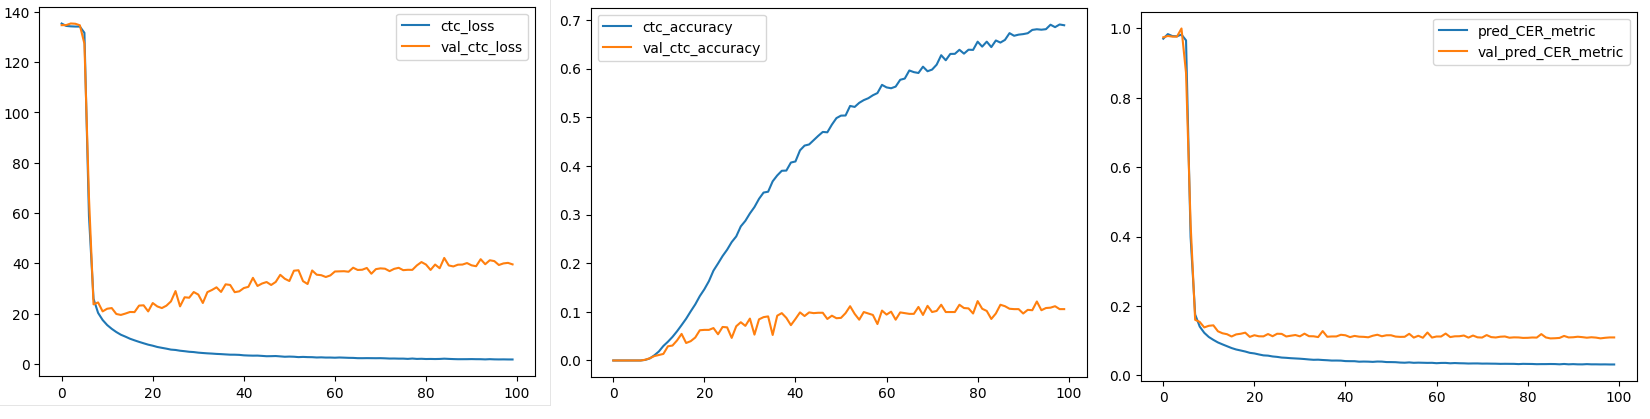
\includegraphics[scale=0.35]{figures/metrics_recog.png}
    \caption{Position-focused Recognition model metrics per epoch \\ (IAM lines + 87 custom samples)}    
    \label{FigPosRecMetrics}
\end{figure}


Figure \ref{FigRecMetrics} presents the evolution of loss, accuracy and CER during recognition model training. The final values are listed in table \ref{TableRecognitionMetrics}. Out of multiple runs on the IAM dataset, the lowest obtained validation CER was 0.08, while it was previously observed the error rate for state of the art methods oscillates around 0.02. Another experimental run with 78 additional images resulted right from the segmentation algorithm was performed on an augmented dataset with generator which changes the offset of input each input. The goal was to ensure the model's robustness when facing different alignments. The validation data contains the same images as the train set, but with altered positions. For this experiment, it was expected for the validation metrics to be the same as the train ones. The results shown in table \ref{TablePositionalRecognition} and figure \ref{FigPosRecMetrics} speak for themselves.


\begin{figure}
    \centering
    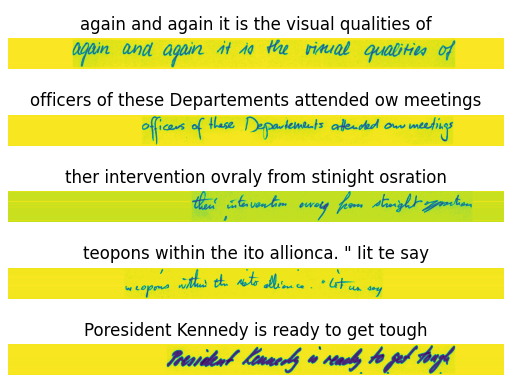
\includegraphics[width=0.7\linewidth]{figures/iam_val_out.png}
    \caption{Recognized text on IAM lines validation data}
    \label{FigIamValOut}
\end{figure}


\begin{table}[htbp]
\begin{center}
\begin{tabular}
{|p{60pt}|p{60pt}|p{100pt}|}
\hline
 Metric  &  Train Value &  Validation value \\
\hline 
Accuracy & 0.6889 & 0.1055 \\ \hline
CER & 0.0309 & 0.1089 \\ \hline

\end{tabular}
\end{center}
\caption{Recognition metrics (pure IAM lines dataset)}
\label{TableRecognitionMetrics}
\end{table}

\begin{table}[htbp]
\begin{center}
\begin{tabular}
{|p{60pt}|p{60pt}|p{100pt}|}
\hline
 Metric  &  Train Value &  Validation value \\
\hline 
Accuracy & 0.8805 & 0.0241 \\ \hline
CER & 0.8267 & 0.0230 \\ \hline

\end{tabular}
\end{center}
\caption{Position-focused recogmition model metrics (IAM lines+ 78 custom samples))}
\label{TablePositionalRecognition}
\end{table}


